\section{Zielsetzung}
\label{sec:Zielsetzung}
In diesem Versuch werden Brückenschaltungen dazu verwendet verschiedene unbekannte Ohm'sche Widerstände, Kapazitäten und Induktivitäten
zu bestimmen. Zudem wird die Wien-Robinson-Brücke dazu verwendet um die Frequenzabhängigkeit dieser Schaltung zu untersuchen. \\
Dabei werden bisher nur in der Theorie benutze Konzepte angewendet, wie beispielsweise die Abgleichbedingung und die Kirchhoff'schen Gesetze.

\section{Theorie}
\label{sec:Theorie}

Brückenschaltungen werden dazu benutzt, durch bereits bekannte Widerstände Unbekannte zu bestimmen. Zu diesen Widerständen zählen
Ohm'sche Widerstände, induktive Widerstände und kapazitative Widerstände. Bei den letzteren Beiden handelt es sich um komplexe
Widerstände. \\
Allgemein werden bei allen folgenden Schaltungen die Kirchhoffschen Gesetze
\begin{equation}
    \sum_k I_k = 0 \\ \label{eqn:K1}
\end{equation}
\begin{equation}
    \sum_k U_k = \sum_k I_k R_k \label{eqn:K2}
\end{equation}
verwendet, wobei bei \autoref{eqn:K2} alle $I_k$ im Uhzeigersinn als positiv und alle gegen den Uhzeigersinn als negativ zu werten sind. \\
Aus diesen grundlegenden Gesetzten \autoref{eqn:K1} und \autoref{eqn:K2} lässt sich die Abgleichbedingung herleiten:
\begin{equation}
    R_1 R_4 = R_2 R_3
\end{equation}
Diese Formel ist nur erfüllt wenn die Brückenspannung minimal wird.
\\

\subsection{Wheatstonesche Brückenschaltung}
 
Die meisten Brückenschaltungen bestehen aus einer Speisespannung $U_S$, bekannten Widerständen, einem unbekannten Widerstand und einem Spannungsmessgerät.
Der einfachste Aufbau besteht aus drei bekannten und einem unbekannten Widerstand, welche wie in \autoref{Abb:Wheatstone} aufgebaut werden.

\begin{figure}
    \centering
    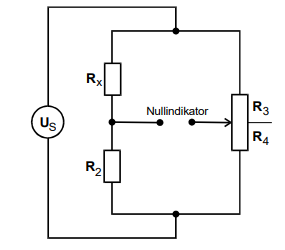
\includegraphics{Wheatstone.png}
    \caption{Wheatstonesche Brückenschaltung}
    \label{Abb:Wheatstone}
\end{figure}

Bei \autoref{Abb:Wheatstone} handelt es sich um eine Wheatstonesche Brückenschaltung. Sie kann sowohl mit Gleichstrom, als auch mit Wechselstrom betrieben werden.
Diese Schaltung wird zur Bestimmung des Widerstands $R_X$ benutzt. Die Widerstände $R_3$ und $R_4$ können in diesem Fall durch ein Potentiometer ersetzt werden,
da nur das Verhätnis der beiden Widerstände relevant zur Bestimmung von $R_X$ ist. \\


\cite{sample}